\documentclass{article}
\usepackage{tikz} 
\usepackage{pgfplots} 
\usepackage{stix}
\usepackage{gillius}
\usepackage[margin=0in, includehead, includefoot, paperwidth=8.625in, paperheight=8.75in]{geometry}
\usetikzlibrary{backgrounds}
\usetikzlibrary{patterns}
\usepackage{microtype}

\begin{document}
\pagenumbering{gobble}


\tikz[remember picture,overlay] \node[inner sep=0pt,%fill=black,opacity=.4
] at (current page.center){\reflectbox{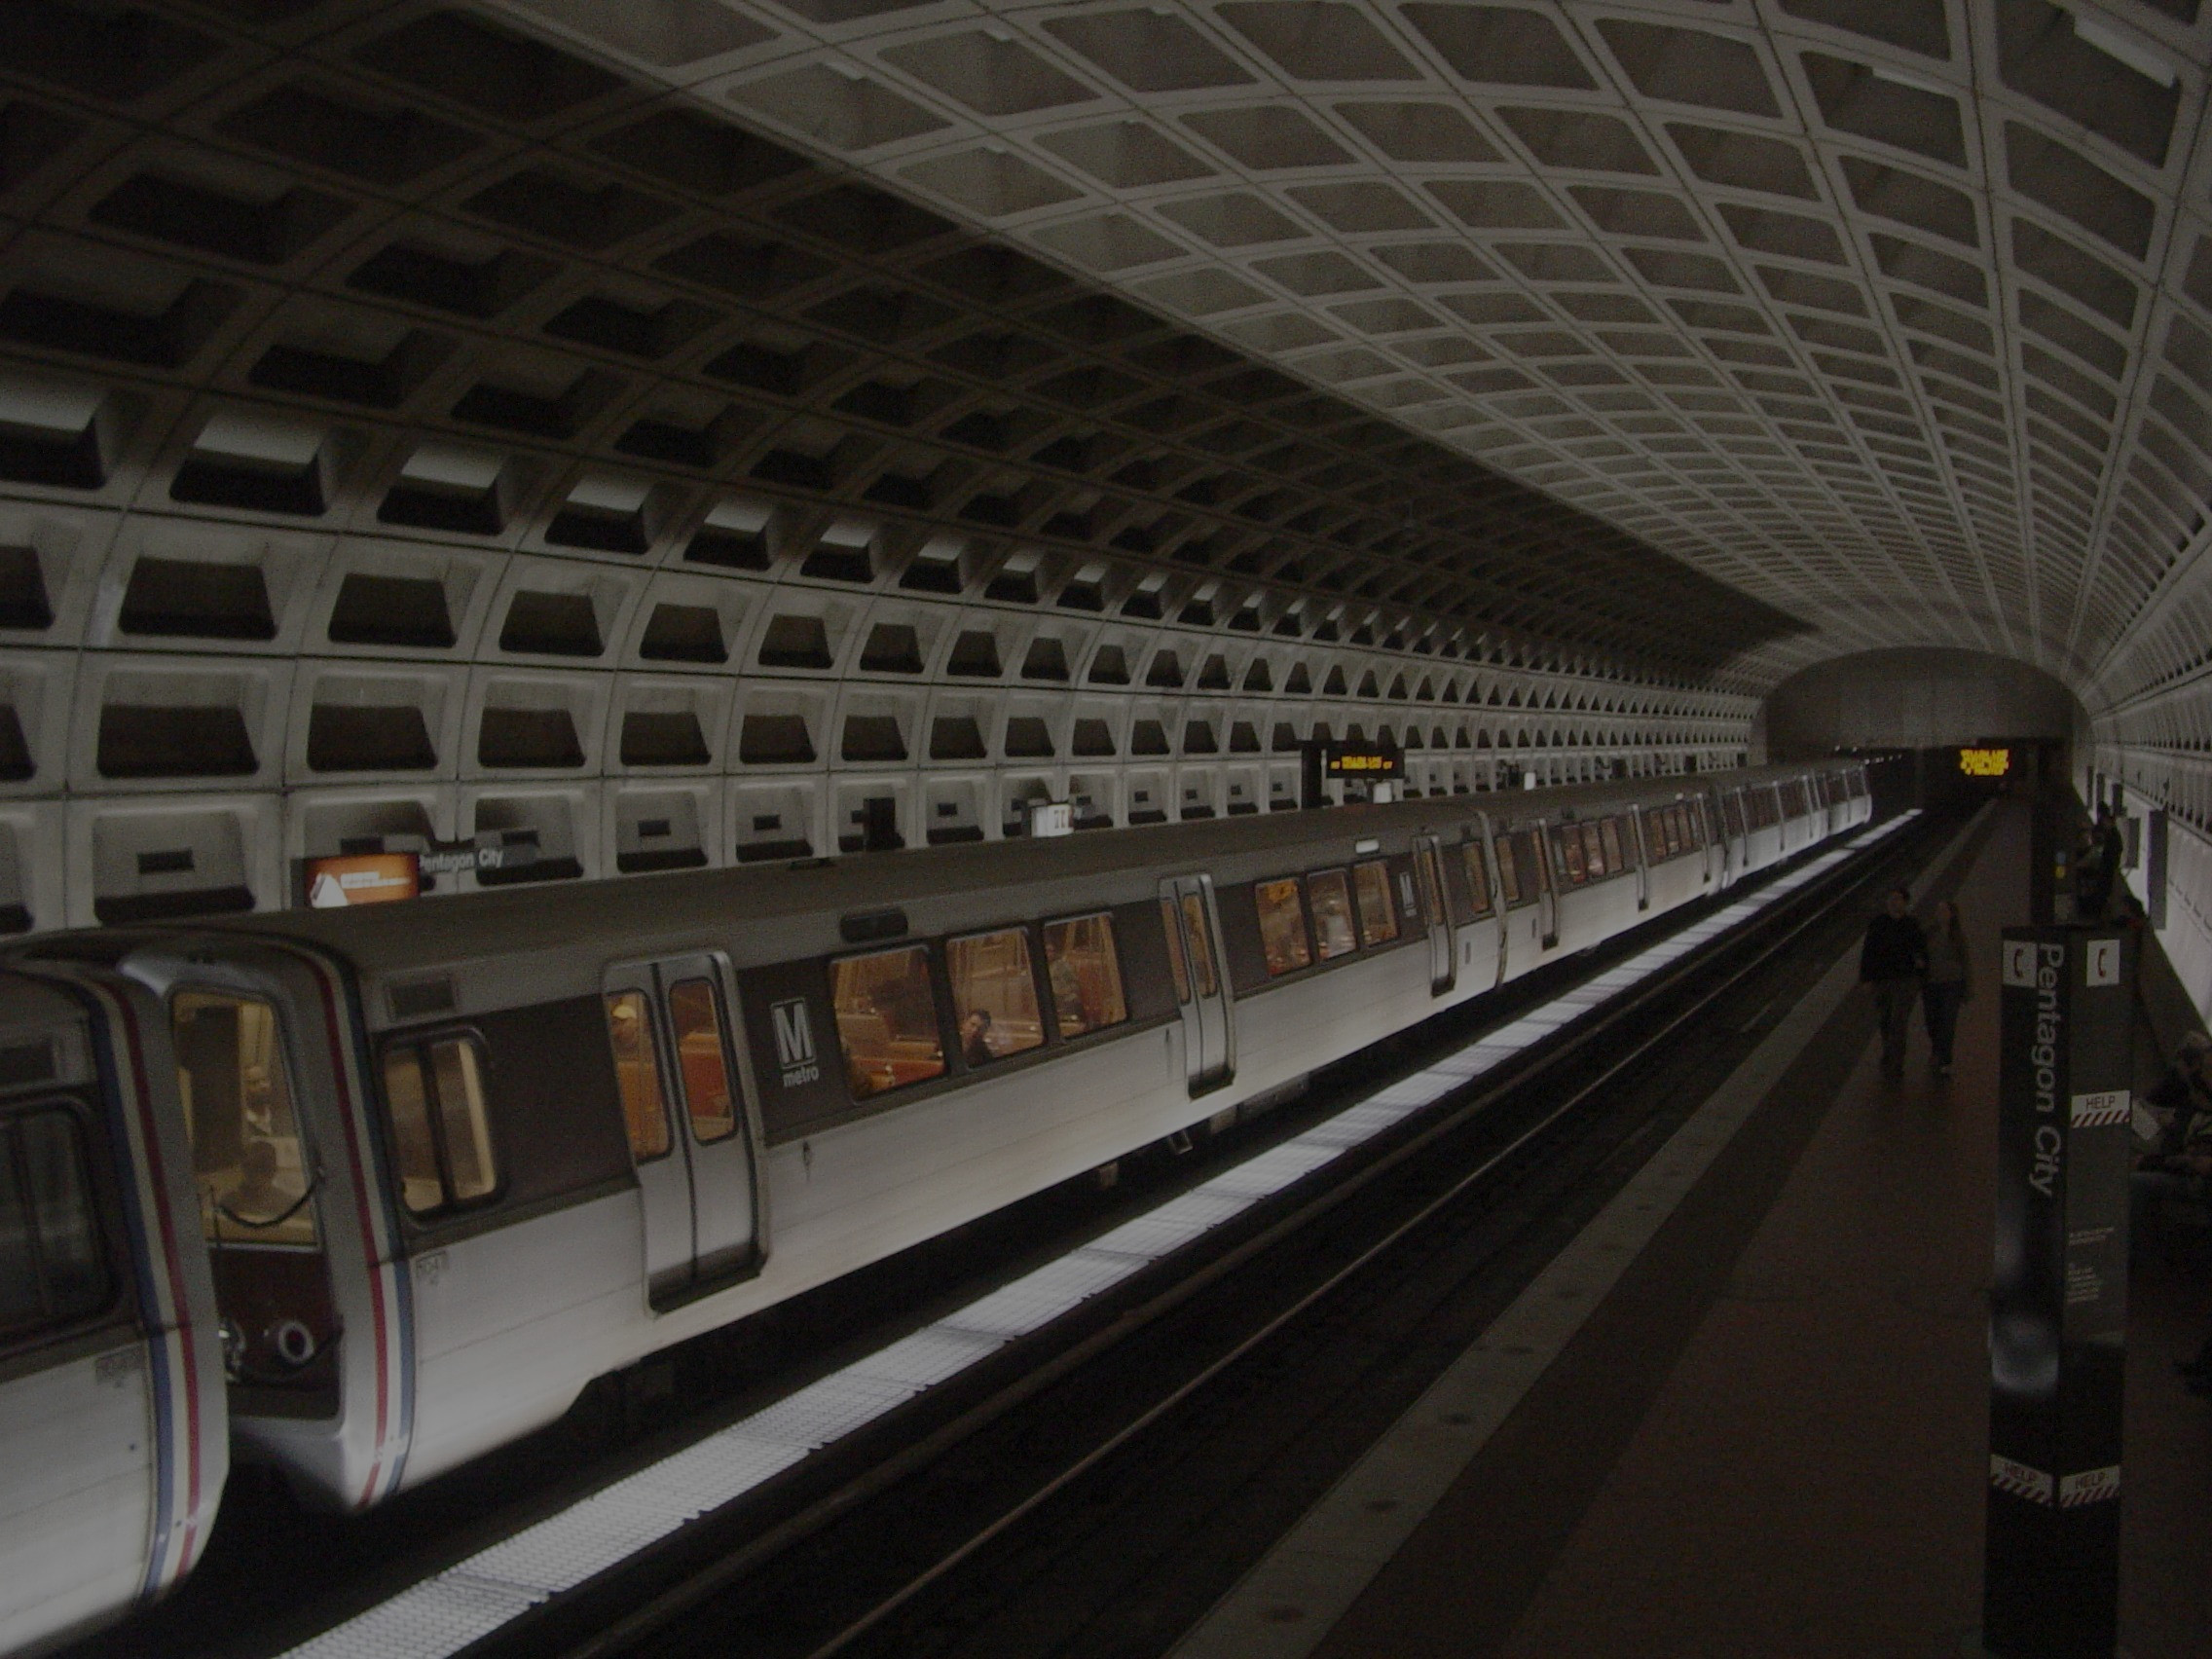
\includegraphics[height=8.75in]{metroStationDark.jpg}}};

%\tikz[remember picture,overlay] \node[inner sep=0pt] at (current page.center){\includegraphics[width=8.625in]{backTemplate.png}};

\vspace{.5cm}

\hspace*{.4in}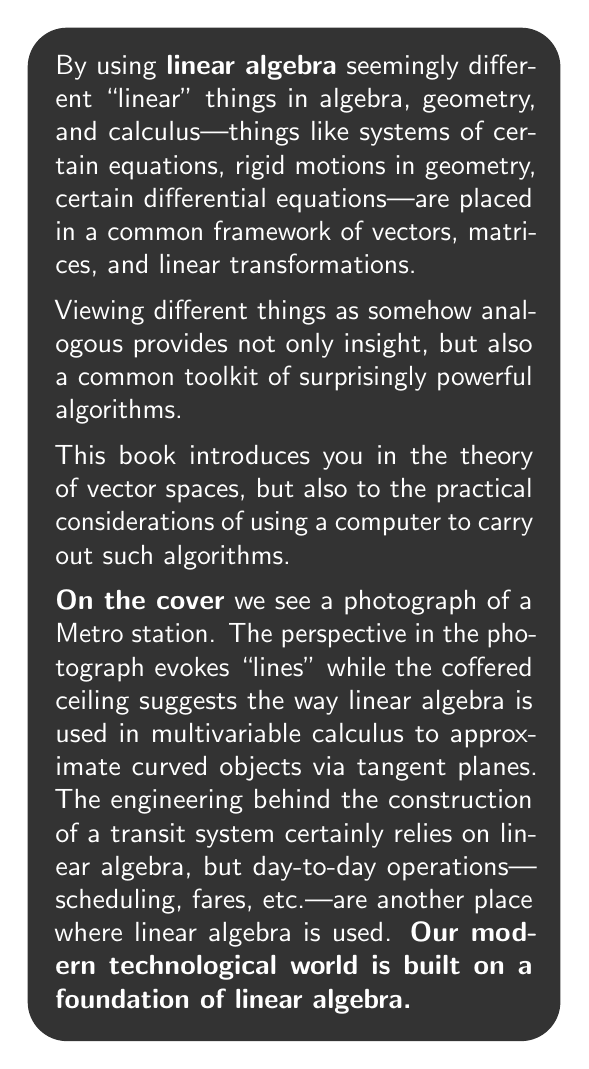
\begin{tikzpicture}
  \node[inner sep=10pt,outer sep=0pt, fill=black, text=white, opacity=.8,text opacity=1,rounded corners=0.5cm]  (box){%
    \begin{minipage}{0.50\textwidth}
      \sffamily\color{white}

      By using \textbf{linear algebra} seemingly different ``linear''
      things in algebra, geometry, and calculus---things like systems
      of certain equations, rigid motions in geometry, certain
      differential equations---are placed in a common framework of
      vectors, matrices, and linear transformations.

      \vspace{1ex}
      
      Viewing different things as somehow analogous provides not only
      insight, but also a common toolkit of surprisingly powerful
      algorithms.

      \vspace{1ex}

      This book introduces you in the theory of vector spaces, but
      also to the practical considerations of using a computer to
      carry out such algorithms.
      
      \vspace{1ex}
      
      \textbf{On the cover} we see a photograph of a Metro station.
      The perspective in the photograph evokes ``lines'' while the
      coffered ceiling suggests the way linear algebra is used in
      multivariable calculus to approximate curved objects via 
      tangent planes.  The engineering behind the construction of a
      transit system certainly relies on linear algebra, but
      day-to-day operations---scheduling, fares, etc.---are another
      place where linear algebra is used.  \textbf{Our modern
        technological world is built on a foundation of linear
        algebra.}

    \end{minipage}
  };
  
  \end{tikzpicture}


\end{document}


